\chapter{Literature Review}
\phantomsection
\label{ch:literature}

\section{Overview}
\phantomsection
\label{sec:ocr-overview}
This chapter provides a comprehensive literature review covering several 
key aspects of Optical Character Recognition (OCR). 
It begins with a definition of OCR, followed by an overview of its technological
 evolution over time. Particular attention is given to the unique challenges 
 associated with Khmer OCR, a low-resource language with complex script characteristics.
  The chapter also explores the significant role of synthetic data in addressing data 
  scarcity for low-resource language processing and dataset development.
   Finally, the chapter concludes by identifying and summarizing the existing 
   research gaps in the current literature, highlighting areas that remain 
   under-explored and underscoring the need for further investigation.


\section{Definition of Optical Character Recognition (OCR)}
\phantomsection
\label{sec:ocr-definition}
Optical Character Recognition (OCR) is a field of computer vision and pattern recognition
 that focuses on the automatic identification and digitization of printed or handwritten 
 text from images, scanned documents, or other visual media \citep{singh2012survey}. 
 OCR systems aim to convert visual representations of text into machine-encoded formats, 
 enabling automated indexing, editing, and data extraction \citep{muaz2015khmerocr}.

Modern OCR technology has evolved significantly from its early rule-based and template-matching
roots to incorporate advanced machine learning techniques, particularly deep learning,
which allow for improved accuracy in character detection, segmentation, and classification across 
diverse languages and scripts.

OCR systems typically consist of several key components: image preprocessing (e.g., noise removal, binarization), text detection, character segmentation, feature extraction, and recognition. These systems must be adapted to handle various font styles, image distortions, complex layouts, and script-specific features. While OCR for Latin-based languages has become highly accurate, extending such systems to non-Latin scripts—such as Khmer—remains a significant research challenge due to unique linguistic and structural characteristics.
   
\section{Khmer Optical Character Recognition (OCR)}
\phantomsection
\label{sec:khmer_OCR_literature}

\citet{CheyFirstOCR} The first significant research on Optical Character Recognition (OCR) 
for Khmer script was proposed in 2006, marking a foundational contribution 
to Khmer language digitization. The study addressed critical challenges 
inherent to Khmer printed characters, notably the variation in character 
shapes across fonts and the high visual similarity between certain 
characters. To overcome these issues, the authors introduced a novel 
recognition method utilizing Wavelet Descriptors. The approach involved 
transforming printed character images into their skeleton forms, 
then converting these skeletons into the temporal domain. Character 
templates were generated using wavelet coefficients from a training set, 
and recognition was performed through a deformable wavelet descriptor 
and a Euclidean distance classifier. The recognition process selected 
the template with the smallest distance to the input character as the 
result. Interestingly, deformation was later excluded from the final 
method due to its adverse impact on distinguishing similar characters. 
Experimental evaluation demonstrated promising results: recognition 
rates of 92.85\%, 91.66\%, and 89.27\% for 22-point, 18-point, and 
12-point font sizes respectively, across 10 Khmer fonts. A second 
test used a 21-page document scanned at varying resolutions 
(150, 300, 600 dpi) and fax inputs, achieving recognition rates 
of 92.99\% at 300 dpi, 88.61\% at 150 dpi, and 80.05\% for faxed documents. 
This pioneering work laid the groundwork for future Khmer OCR systems 
and remains a landmark study in Khmer script recognition.

\citet{Sok&Taing2014} The second significant research on 
Khmer Optical Character Recognition (OCR) introduces a Support 
Vector Machine (SVM)-based approach for printed Khmer character 
recognition in bitmap documents. Given the inherent complexity 
of the Khmer script—which includes 74 alphabets and the potential 
for up to five vertical levels in word compounds—the study focuses 
on identifying the most effective SVM kernel for classification.

The proposed method evaluates three SVM kernels: Gaussian, Polynomial, 
and Linear. Rather than training on large datasets, the system adopts 
a modular approach, segmenting characters into smaller parts. Each 
segment is transformed into a binary matrix, with 1s representing 
black pixels and 0s for whitespace. Feature extraction is applied 
to these matrices for SVM training and classification.

Following recognition, post-processing rules are employed to merge 
character clusters and correct common misclassifications based on 
character levels. The training utilized one font ("Khmer OS Content") 
at 32pt and tested recognition performance across three font sizes 
(28pt, 32pt, and 36pt). The results demonstrated strong accuracy:
\begin{itemize}
  \item 98.17\% for 28pt,
  \item 98.62\% for 32pt,
  \item 98.54\% for 36pt.
\end{itemize}

The Gaussian kernel outperformed the other kernels, confirming its 
suitability for Khmer character recognition. This study highlights 
the effectiveness of machine learning-based OCR for complex scripts 
like Khmer and marks a major advancement over earlier template-based 
systems.

\citet{Meng_Hann_2014} proposed a Khmer Character Recognition (KCR) 
system utilizing artificial neural networks to address the complexity 
of recognizing individual Khmer script characters. Developed in a 
MATLAB environment, the system integrates a Self-Organizing Map (SOM) 
for unsupervised clustering with a Multilayer Perceptron (MLP) 
trained via the backpropagation algorithm for supervised classification. 
The recognition process follows a two-stage pipeline: first, the input 
image—resized to 20×20 pixels—is categorized by the SOM into one of 
nine coarse groups. Then, each group is assigned to a dedicated MLP 
model, which performs fine-grained classification into one of 82 
target classes, including Khmer consonants, vowels, and numerals. 
This modular approach aims to enhance classification efficiency by 
narrowing the decision space for each MLP. The system achieved an 
average recognition accuracy of 65\% on the training dataset and 
30\% on the testing dataset, highlighting both the potential and 
the challenges of neural network-based Khmer OCR at the time.

\citet{Muaz2015} This study presents a comprehensive OCR system for 
printed Khmer text using the HTK Toolkit, covering the full 
pipeline of pre-processing, segmentation, recognition, and mapping. 
The system is tailored for the widely used Limon S1 font at 22pt and 
introduces a structural segmentation approach that decomposes 
characters into five categories: Main Body, SuperScript, SubScript, 
CCDown, and Complex Character (CC). Feature extraction relies on 
vertical framing and Discrete Cosine Transform (DCT), with 
classification handled by Hidden Markov Models (HMMs). 
The system was trained on over 35,000 labeled shape samples and 
evaluated on 10 pages of scanned newspaper text, achieving an 
overall recognition rate of 96.34\%. While the results are promising, 
the system is limited by its reliance on a single font style and size, 
making it less robust to font variation. Additionally, recognition 
performance drops for complex shapes like CC (70.88\%) and depends 
heavily on manually crafted mismatch and rule files for post-processing, 
indicating scalability and generalization challenges for real-world 
applications involving diverse document types and fonts.

\citet{Valy_8563219} proposed a character-level Convolutional Neural 
Network (CNN) model for recognizing ancient Khmer script from digitized 
palm leaf manuscripts. The study focuses on two core tasks: 
isolated character recognition and word-level glyph localization. 
For the character recognition task, a CNN architecture comprising 
three convolutional blocks followed by a linear classifier was 
developed. The output layer of the network predicts one of 106 
character classes, achieving a reported test accuracy of 95.96\%. 
In addition to CNNs, the study also explores other neural 
architectures including LSTM-RNN and hybrid CNN-RNN models. 
For the word/text image recognition task, the authors leveraged 
both one-dimensional and two-dimensional RNNs to handle the complex 
spatial structure of Khmer script and to localize glyphs within 
variable-length text patches. This research highlights the potential 
of deep learning approaches in historical Khmer OCR, particularly in 
handling the challenges posed by degraded manuscripts and complex 
writing structures.

\citet{Annanurov_2018} conducted a pilot study on Khmer handwritten 
symbol recognition, focusing on the use of Convolutional Neural 
Networks (CNNs) for digitizing large-scale handwritten document corpora. 
The study used image data from six handwriting datasets containing 
33 Khmer consonants and 17 vowels, forming a total of 561 syllables. 
For consonant recognition, the authors trained 33 individual CNNs—one 
for each root radical—which were later integrated into a recognition 
assembly. The performance of the CNN-based model was evaluated against 
two alternative systems: an artificial neural network (ANN) using the 
full feature set, and another ANN with reduced feature dimensions. 
Feature extraction techniques such as two-dimensional Fourier 
transformation (FT2D) and Gabor filters were employed for dimensionality 
reduction. The CNN-based approach achieved a recognition accuracy of 
up to 94.85\%, outperforming the ANN-based models. However, the system 
was limited to recognizing only Khmer consonants, without support for 
vowel or syllable-level recognition.

\citet{sokphyrum2019khmer} fine-tuned the Tesseract OCR engine 
(version 4.0) to improve recognition of Khmer Unicode and legacy 
Limon fonts. Tesseract 4.0 employs a deep convolutional recurrent 
neural network with a connectionist temporal classification (CTC) 
loss function and attention mechanism, enabling it to recognize entire 
text-line images. The fine-tuning process involved training on 14 Khmer 
Unicode fonts and 20 pre-Unicode Limon fonts (all at 12pt size). 
The ISRI Analytic Tools were used to evaluate OCR accuracy at both 
the character level (CHL) and cluster level (CLL) by comparing OCR 
outputs to ground truth text. The Khmer pre-trained engine achieved 
an average accuracy of 87.49\% at the character level and 89.43\% at 
the cluster level on Unicode fonts, while legacy Limon fonts yielded 
a significantly lower median accuracy of 62.27\%. After fine-tuning, 
recognition accuracy reached up to 90\% for specific fonts, demonstrating 
the potential of domain-specific adaptation to enhance OCR performance 
for complex scripts like Khmer.

\citet{buoy2021seq2seq} Despite progress in OCR for high-resource languages, 
Khmer OCR still faces significant challenges due to its complex script structure 
involving stacked consonants, diacritics, and positionally variable vowels. Traditional 
Khmer OCR methods relied on segmentation-based pipelines and character-level 
classification, often struggling with noisy or long text-line images. This paper 
introduces one of the first end-to-end solutions for Khmer OCR using a 
Sequence-to-Sequence (Seq2Seq) architecture with an attention mechanism. The encoder 
consists of residual convolutional blocks and bidirectional GRU layers that extract 
feature sequences from text-line images, while the decoder generates characters one-by-one 
using attention to focus on relevant parts of the image. The model is trained on a large 
synthetic dataset generated from the Khmer ALT corpus using multiple fonts and aggressive 
augmentation techniques. Evaluated on a 3000-image test set, the model achieves 1\% 
character error rate (CER) and 9\% word error rate (WER), significantly outperforming 
the Khmer Tesseract OCR engine, which achieves 3\% CER and 26\% WER. Additionally, 
the model demonstrates robustness to image noise, font variations, and camera-captured texts, 
highlighting the effectiveness of attention-based Seq2Seq models in low-resource OCR tasks.

\citet{Buoy2022} Khmer printed character recognition presents significant 
challenges due to the script's complex structure, including stacked consonants, 
dependent vowels, and diacritics placed in various positions. Traditional approaches, 
such as SVMs, wavelet-based templates, and CNNs, have largely focused on recognizing standalone 
characters and depend heavily on accurate segmentation, making them less robust for noisy or 
continuous text-line images. Tesseract OCR, though improved with deep neural networks 
and CTC loss, still performs poorly on heavily augmented images with a reported Character 
Error Rate (CER) of 35.9\%. In contrast, the reviewed study introduces an end-to-end 
attention-based Sequence-to-Sequence (Seq2Seq) model that directly maps entire text-line 
images to character sequences without needing pre- or post-processing. Trained on 3 million 
synthetically generated and augmented images across multiple Khmer fonts, the model 
achieved a CER of 0.7\% on noisy images and 0.24\% on clean images, significantly 
outperforming existing methods and demonstrating the effectiveness of attention mechanisms 
and deep learning for low-resource scripts like Khmer.

\citet{nom2024khmerst} The Khmer script poses significant challenges for scene text detection 
and recognition due to its complex structure involving stacked consonants, multiple diacritics, 
subscript characters, and the lack of explicit word boundaries. To address the scarcity of 
resources for this low-resource language, this study introduces KhmerST, the first annotated 
scene-text dataset for the Khmer language, consisting of 1,544 real-world images captured 
from various public settings in Cambodia. Unlike existing synthetic Khmer datasets, 
KhmerST includes indoor and outdoor images with diverse fonts, orientations, and 
background conditions, and provides polygon-based line-level annotations for more accurate 
localization. Benchmarking with YOLO models shows that YOLOv8 performs best in detection 
tasks due to its ability to handle small and variable text elements, while in recognition 
tasks, both TrOCR and Tesseract perform poorly, with TrOCR achieving CER of 0.90 and 
Tesseract CER of 1.30, highlighting the need for Khmer-specific OCR models. The study 
underscores the gap between current OCR systems and the needs of Khmer script recognition, 
calling for future research on synthetic data generation, Khmer-aware model design, 
and multimodal approaches to improve accuracy in real-world applications.

\citet{Rina2025} This research addresses the challenge of Khmer textline recognition, 
which is particularly difficult due to the absence of spaces between words in the Khmer script. 
Unlike Latin-based languages, this structure requires recognition to be performed at the textline level, 
leading to high latency when using autoregressive (AR) decoders that predict one character at a 
time while considering previous characters. In contrast, non-autoregressive (NAR) decoders can decode 
all characters in parallel but lack awareness of character dependencies, resulting in lower linguistic 
accuracy. To solve this, the authors propose an efficient Khmer textline recognition method using an NAR 
decoder, enhanced by Khmer-specific subword modeling. Instead of predicting single characters, the model 
recognizes character clusters (subwords), capturing the syntactic, morphological, and orthographic 
structure of the language implicitly. This design retains the speed of NAR models while improving accuracy. 
Experimental results show that the proposed method outperforms the character-level NAR baseline 
in accuracy and matches or exceeds the AR baseline while maintaining lower latency. However, 
the abstract does not report detailed accuracy or metrics, and access to full experimental results 
requires a subscription, limiting transparency for non-subscribers. This work contributes an 
important step toward faster and more linguistically aware Khmer OCR by bridging the gap between 
speed and accuracy in scene text recognition.
    

\subsection{Advancements in Khmer OCR (2021-Present)}
\phantomsection
\label{sec:advancements-in-khmer-ocr}

The new Khmer OCR system is built using a sequence-to-sequence (Seq2Seq) 
deep learning model with attention. Instead of recognizing each character separately, 
the model looks at a whole line of text and understands it as a sequence, 
just like how we read. It starts with an encoder that uses convolutional layers 
to extract visual features from the image and then passes these features 
through a Gated Recurrent Unit (GRU), which captures the order of the characters.

The decoder then takes this information and generates the output text, one character 
at a time. With the help of an attention mechanism, the decoder can focus on different 
parts of the image while predicting each character. This allows the model to handle 
long text lines and various font styles more effectively.

The model was trained on thousands of computer-generated Khmer text images using seven 
common fonts. On a test set of 3,000 images, it achieved a character error rate (CER) 
of only 1\% \citep{buoy2021seq2seq}, which is significantly better than the 3\% 
\citep{buoy2021seq2seq} CER from Tesseract OCR for Khmer. 
This shows the model's high accuracy and reliability.

Compared to older OCR tools like Tesseract, which treat text as a series of separate 
characters, this new end-to-end model sees the text as a whole sequence. 
This helps it better understand context and spacing. It also adapts better 
to different fonts and styles, especially in complex scripts like Khmer. 
The attention mechanism is a major improvement because it lets the model decide 
where to "look" in the image while decoding, which improves accuracy in challenging cases.

In short, this Khmer OCR model uses modern AI to provide faster, smarter, and 
more accurate text recognition, especially for a language that has been 
underserved in OCR research.

\begin{figure}[ht]
    \centering
    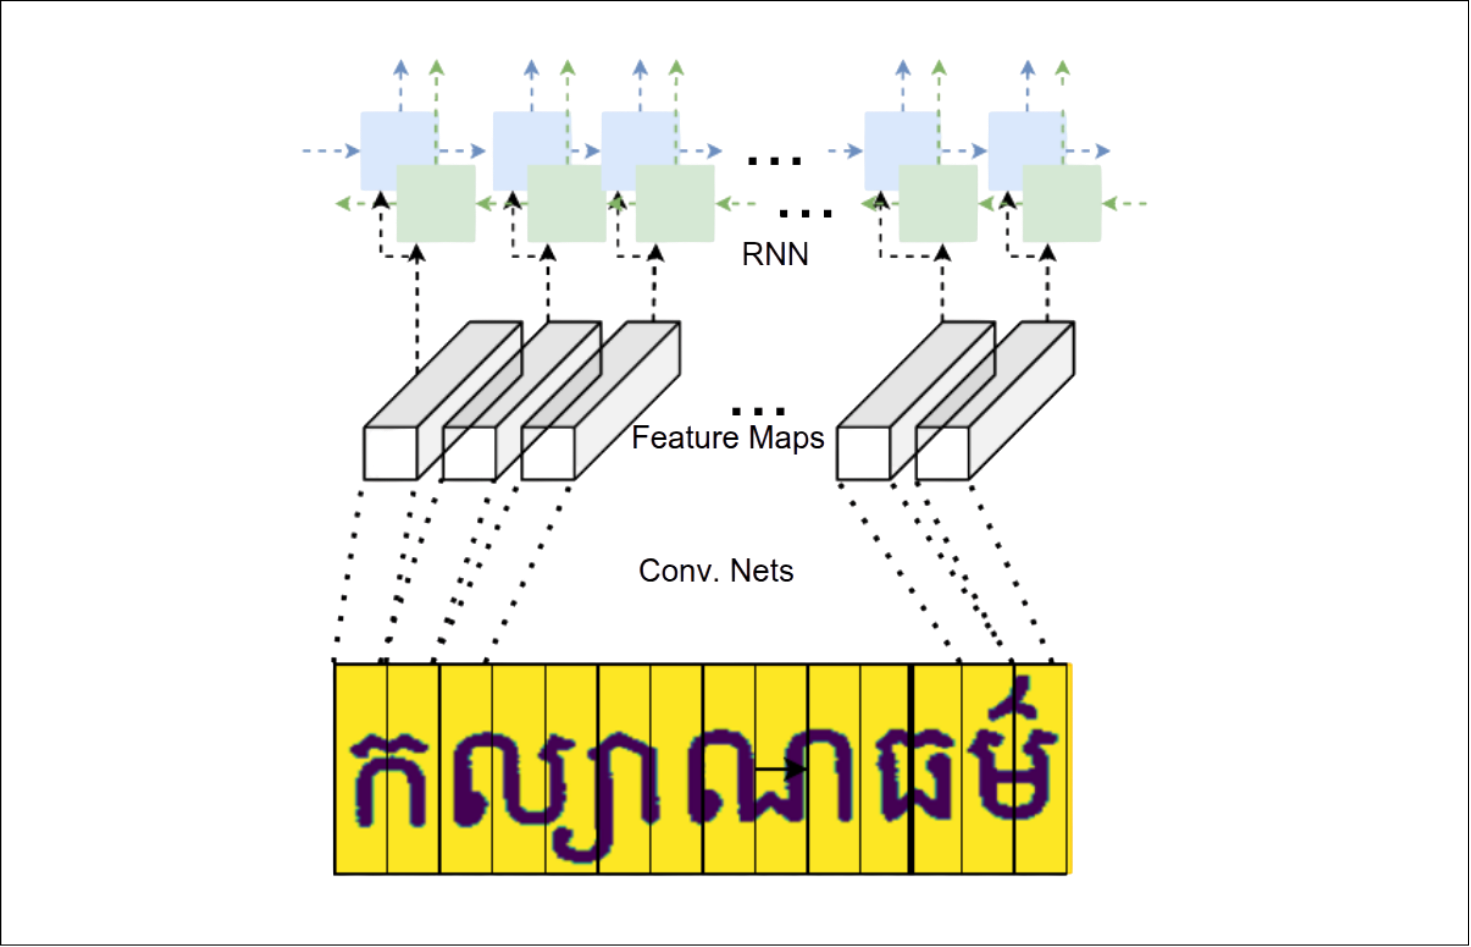
\includegraphics[width=\textwidth]{figures/bouy_rina_end_to_end_khmer_ocr.png}
    \caption{Illustration of the end-to-end Khmer OCR system proposed by Bouy and Rina,
    which combines a feature extractor, a sequence-to-sequence model,
     and a post-processing module to achieve high accuracy in recognizing Khmer text. \citep{buoy2021seq2seq}}
    \label{fig:bouy-rina-end-to-end-khmer-ocr}
\end{figure}


\section{Challenges in Khmer OCR}
\phantomsection
\label{sec:datasets}

One of the biggest challenges in Khmer OCR lies in the complexity of the Khmer script. 
Unlike Latin-based languages,  Khmer characters can be stacked and combined using 
subscript consonants (Coeng), \citep{buoy2021seq2seq} diacritics, and various vowel positions. These components 
can appear above, below, to the left or right, or even surround the base character. 
This spatial variability significantly complicates the segmentation and recognition 
process, especially for systems that rely on isolated character analysis.

Khmer script is written in a wide range of fonts, each with its own style and visual 
characteristics. \citep{buoy2021seq2seq} These differences affect how characters are formed and connected, 
making it difficult for OCR models to generalize well across different typefaces. 
An effective OCR system must therefore be font-invariant and capable of accurately 
recognizing characters in any common or uncommon font.

Khmer is considered a low-resource language in the fields of natural language 
processing and OCR. This means there are limited publicly available datasets, 
pretrained models, and tools. As a result, researchers face difficulty in 
training robust models without generating synthetic data or heavily augmenting 
existing datasets.

Older Khmer OCR systems typically rely on explicit character segmentation, 
breaking down the text into individual symbols before recognition. 
This approach is prone to failure when applied to real-world images that 
contain noise, uneven spacing, or distorted characters. \citep{buoy2021seq2seq} Since Khmer characters 
often overlap or combine, segmentation errors are common and negatively affect 
recognition accuracy.

\begin{figure}[ht]
    \centering
    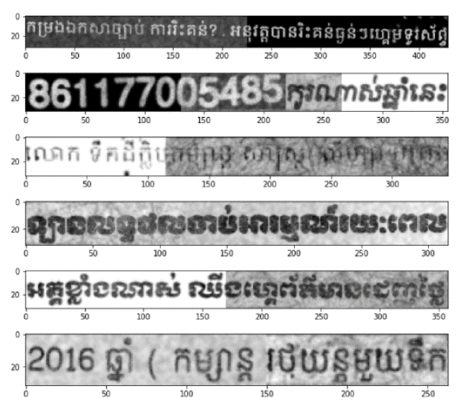
\includegraphics[width=\textwidth]{figures/overlap_segmentation.png}
    \caption{Khmer characters can overlap or combine in special ways, 
    making explicit segmentation prone to errors. \citep{buoy2021seq2seq}}
    \label{fig:overlap-segmentation}
\end{figure}

Prior Khmer OCR efforts have primarily focused on isolated character recognition 
and manual pre/post-processing steps. These systems are limited in their ability to 
recognize full words, phrases, or sentences. In contrast, an end-to-end solution can 
read an entire line of text and generate output in a single forward pass, 
improving speed, simplicity, and accuracy. \citep{buoy2021seq2seq}



\section{Role of Synthetic Data}
\phantomsection
\label{sec:dl-models}

To overcome the limitations of Khmer being a low-resource language, 
the authors created a large-scale synthetic dataset of Khmer \textbf{text-line} 
images using the open-source \textbf{text2image} tool provided by the Tesseract OCR engine.

The dataset was generated from a text corpus containing numbers, words, phrases, 
and full sentences in Khmer. \citep{buoy2021seq2seq} This corpus provided diverse linguistic content 
for rendering text-line images.

Multiple common Khmer fonts were used to render each item from the corpus. 
The variation in fonts helped train the model to be font-invariant and improve 
generalization across different writing styles.

The \textbf{text2image} tool was used to convert each text entry from the corpus into a 
grayscale image. The width and height of each image varied based on the text 
length and presence of stacked or subscript characters. All images were 
resized to a common height of 32 pixels to match the input size required 
by the neural network.

To simulate real-world challenges and improve the model's robustness, 
extensive data augmentation was applied \citep{buoy2021seq2seq} :
    \begin{itemize}
        \item Gaussian blurring
        \item Dilation and erosion
        \item Blob noise and speckle noise
        \item Multi-scale noisy backgrounds
        \item Random concatenation of augmented images
        \item Rotational and geometric distortions
    \end{itemize}

Each augmentation had a 50\% \citep{buoy2021seq2seq} chance of being applied to a given image, and multiple augmentations could be combined on a single image. This ensured that the model was trained on a wide range of noisy and distorted text scenarios.

The final synthetic dataset consisted of millions of images representing words, 
phrases, and sentences across different fonts and styles.

\section{Summary of Research Gaps}
\phantomsection
\label{sec:research-gaps}

This section identifies the key research gaps in the current literature on 
Khmer OCR technology. Despite advancements, several areas remain under-explored:

\begin{itemize}
    \item \textbf{Data Scarcity:} There is a lack of large-scale annotated datasets for Khmer text, which limits the training and evaluation of OCR models.
    \item \textbf{Complex Script Features:} The unique characteristics of Khmer script, such as character stacking and the absence of word boundaries, are not fully addressed by existing models.
    \item \textbf{Font Variability:} Current OCR systems struggle with the wide variety of fonts used in Khmer documents, affecting recognition accuracy.
    \item \textbf{Real-world Document Conditions:} Many models are not robust to the noise, distortions, and variations found in real-world documents.
\end{itemize}

Addressing these gaps is crucial for developing more effective and reliable Khmer OCR solutions.

